\documentclass{beamer}
\usepackage[utf8]{inputenc}
\usepackage[T1]{fontenc}
\usepackage[slovene]{babel}
\usepackage{lmodern}

\usepackage{amsfonts,url, amsthm}
\usepackage{palatino}
\usepackage{graphicx, tikz, array}

\usefonttheme{professionalfonts}
\mode<presentation>
{
  \usetheme{Berlin}
  \usecolortheme{default}
  \useoutertheme{infolines}
  \useinnertheme[shadows]{rounded}
}

\newtheorem{izr}{Izrek}
\newtheorem{posl}{Posledica}[izr]

\newcounter{defcount}
\newcounter{opombe}
\newcounter{zgledcount}

\newenvironment{opomba}{\begin{flushleft}\stepcounter{opombe}\textbf{Opomba \arabic{opombe}:}}{\hfill\end{flushleft}}
\setlength{\parindent}{0mm}

\newenvironment{zgled}{\begin{flushleft}\stepcounter{zgledcount}\textbf{Zgled \arabic{zgledcount}:}}{\hfill\end{flushleft}}
\setlength{\parindent}{0mm}

\newenvironment{definicija}{\begin{flushleft}\stepcounter{defcount}\textbf{Definicija \arabic{defcount}:}}{\hfill\end{flushleft}}
\setlength{\parindent}{0mm}

\newcommand{\naslov}[1]{\textit{#1}}
\newcommand{\abs}[1]{\ensuremath{\lvert #1 \rvert}}
\newcommand{\mth}[1]{\ensuremath{\mathbb{#1}}}
\newcommand{\R}{\mth{R}}
\newcommand{\Z}{\mth{Z}}
\newcommand{\Zp}{\mth{Z}^{+}}
\newcommand{\N}{\mth{N}}
\newcommand{\No}{\mth{N}_0}
\newcommand{\C}{\mth{C}}
\newcommand{\Qu}{\mth{Q}_u}
\newcommand{\Qo}{\mth{Q}}
\newcommand{\pojem}[1]{\emph{#1}}
\newcommand{\con}{\ensuremath{\mathscr{C}}}
\newcommand{\padex}[2]{\ensuremath{{#1}^{\underline{#2}}}}
\newcommand{\rastx}[2]{\ensuremath{{#1}^{\bar{#2}}}}
\newcommand{\map}[3]{\ensuremath{{#1}: {#2} \rightarrow {#3}}}
\newcommand{\pra}[3]{{#1}{\ast}({#2}) = {#3}}

\title[Fermatov poslednji izrek za n=4]{Fermatov poslednji izrek za n=4 in sorodni problemi}

\author{Jimmy Zakeršnik}

\institute[FMF, UL] % (optional, but mostly needed)
{
  Oddelek za Matematiko\\
  Fakulteta za matematiko in fiziko\\
  Univerza v Ljubljani
}

\date[16.5.2019]{Predstavitev seminarske naloge, 16.\ maj 2019, Ljubljana}


%\beamerdefaultoverlayspecification{<+->}


\begin{document}


%%% NASLOVNA STRAN %%%%%%%%%%%

\begin{frame}
  \titlepage{}
\end{frame}

%%%%%%%%%%%%%%%%%%%%%%%%%

\begin{frame}
\frametitle{Motivacija}
\begin{figure}[h]
		\centering
		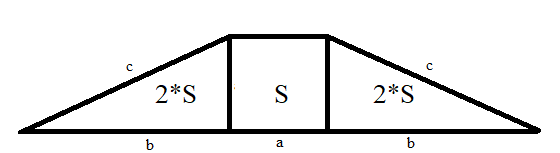
\includegraphics[scale=0.75]{Motivacijska_slika}
		\caption{Skica modela, ki ga želimo sestaviti. $a$, $b$ in $c$ so pozitivna cela števila, $S$ pa površina kvadrata.}
		\label{fig:mot}
\end{figure}
\end{frame}

\begin{frame} 
\onslide<1-2>{
\begin{block}{Izrek (Fermatov poslednji izrek)}
	Naj bo $n$ celo število, ki je (strogo) večje od 2 ($n > 2$). Tedaj enačba $ x^n + y^n = z^n $ nima netrivialnih celoštevilskih rešitev $x, y, z \in \Z$
  \end{block}
}
\onslide<2>{Nas zanima poseben primer $n = 4$}
  
\end{frame}

%%%%%%%%%%%%%%%%%%%%%%%%%

\begin{frame}
	\frametitle{Metoda neskončnega spusta}

	\begin{block}{Pomnimo:}
		Po Peanovih aksiomih, ima množica pozitivnih celih števil $\Zp$ (oz. naravnih števil $\N$) najmanjši element. Drugače povedano, $\Zp$ je navzdol omejena množica.
	\end{block}

\end{frame}

\begin{frame}

\begin{block}{Metoda neskončnega spusta}
	Najpogosteje jo uporabljamo da dokažemo, da neka enačba nima celoštevilskih rešitev:
	
	\begin{itemize}
		\item Predpostavimo, da obstaja neka celoštevilska rešitev $a_1$,
		\pause
		\item pokažemo, da za predpostavljeno rešitev obstaja še ena celoštevilska rešitev $a_2$,
		\pause
		\item postopek ponavljamo in pridobljene rešitve razvrstimo po velikosti s pomočjo preslikave $\map{f}{\Z}{\Zp}$ (npr. $f: x \mapsto\abs{x}$),
		\pause
		\item dobimo neskončno padajočo verigo,
		\pause
	\end{itemize}
	\[
	f(a_1) > f(a_2) > f(a_3) > f(a_4) > \ldots
	\]
	\begin{itemize}
		\pause
		\item protislovje z dejstvom, da so $\Zp$ navzdol omejena.
	\end{itemize}
	
\end{block}

\end{frame}


\begin{frame}
  \frametitle{Primeri uporabe metode}

\onslide*<1->{\begin{block}{Izrek:}
	Ne obstajajo takšna cela števila $x, y ~\text{in}~ z$, ki netrivialno rešijo enačbo $x^3 + py^3 + p^2z^3 = 0$, kjer je $p$ poljubno praštevilo.
\end{block}}

\onslide<2->{\begin{block}{Izrek:}
	Naj bo $d$ celo število, ki ni popolni kvadrat (torej ne obstaja takšno celo število $k$, da bi veljalo $d=k^2$. Potem je $\sqrt{d}$ iracionalno število.
\end{block}}

\end{frame}
%%%%%%%%%%%%%%%%%%%%%%%%%

\begin{frame}
\frametitle{Fermatov poslednji izrek za $n=4$}
\onslide<1->{\begin{block}{Definicija:}
	Pitagorejska trojica je sestavljena iz treh celih števil $a, b, c \in \Z$, za katera velja $a^2 + b^2 = c^2$. Če so $a, b~\text{in}~c$ paroma tuja si števila, pravimo, da je trojica \textbf{primitivna}. Pitagorejsko torjico števil $a, b~\text{in}~c$ označimo z $(a, b, c)$.
\end{block}}

\onslide<2->{\begin{block}{Izrek:}
		Naj bo $(a, b, c)$ Pitagorejska trojica in $d$ neko pozitivno celo število. Potem je ploščina trojici pripadajočega pravokotnega trikotnika enaka dvakratniku ploščine kvadrata s stranico dolžine $d$ natanko tedaj, ko obstaja netrivialna celoštevilska rešitev enačbe $x^4 + y^4 = z^2$
\end{block}}

\end{frame}

%%%%%%%%%%%%%%%%%%%%%%%%%

\begin{frame}
\onslide<1->{\begin{block}{Definicija:}
		Primitivna rešitev, za enačbo $a^2 + b^2 = c^2$, kjer so $a, b~\text{in}~c$ pozitivna cela števila in $b$ sodo (brez škode za splošnost) se glasi:
		\[
		a = k^2 - l^2, b=2kl, c = k^2 + l^2,
		\]
		kjer je $k$ večji od $l$ ter sta si $k$ in $l$ tuji števili različnih parnosti ($gcd(k, l) = 1, k \not\equiv l~mod~2$)
		
\end{block}}

\onslide*<2->{\begin{block}{Izrek:}
		\label{izr:fer}
		Enačba $x^4 + y^4 = z^2$ ni rešljiva v pozitivnih celih številih.
\end{block}}

\end{frame}

%%%%%%%%%%%%%%%%%%%%%%%%%

\begin{frame}
  \frametitle{Nekaj posledic}

\onslide<1->{\begin{block}{Posledica:}
		\label{pos:ena}
		Za vsako trojico racionalnih števil $(x, y, z)$, ki rešijo enačbo $x^4 + y^4 = z^2$ velja, da je bodisi $x$, bodisi $y$ enak $0$.
	\end{block}}

\onslide<2->{\begin{block}{Posledica:}
		\label{pos:dva}
		Edini racionalni rešitve enačbe $y^2 = x^4 + 1$ sta $(0, \pm1)$.
\end{block}}

\onslide<3->{\begin{block}{Posledica}
		\label{pos:tri}
		Edini racionalni rešitvi enačbe $2y^2 = x^4 - 1$ sta $(\pm1; 0)$.
\end{block}}

\onslide<4->{\begin{block}{Posledica}
		\label{pos:stiri}
		Edina racionalna rešitev enačbe $y^2 = x^3 + x$ je $(0, 0)$.
\end{block}}

\end{frame}
%%%%%%%%%%%%%%%%%%%%%%%%%
\begin{frame}
  \frametitle{Viri}

\begin{itemize}
	\item K. Conrad, {\em Proofs by Descent},
	\url{http://www.math.uconn.edu/~kconrad/blurbs/ugradnumthy/descent.pdf}
	
	\item {\em Pythagorean triple},	\url{https://en.wikipedia.org/wiki/Pythagorean_triple}
	
	\item {\em Proof by infinite descent}, \url{https://en.wikipedia.org/wiki/Proof_by_infinite_descent}
	
	\item {\em Well-ordering principle}, \url{https://en.wikipedia.org/wiki/Well-ordering_principle}
	
	\item {\em Peano axioms}, \url{https://en.wikipedia.org/wiki/Peano_axioms}


\end{itemize}

\end{frame}
\end{document}
